\documentclass{journal}
\usepackage{graphicx}
\usepackage{siunitx}
\usepackage{float}
\usepackage{caption}


\begin{document}
\title{AP Calculus Final Project}
\author{Joshua Morin-Baxter, Alan Zhu, Nathan Wiley, and George Hong}
\date{\today}

\maketitle

\part{Wind Angle vs. Wind Velocity}
\begin{figure}[H]
  \centering
  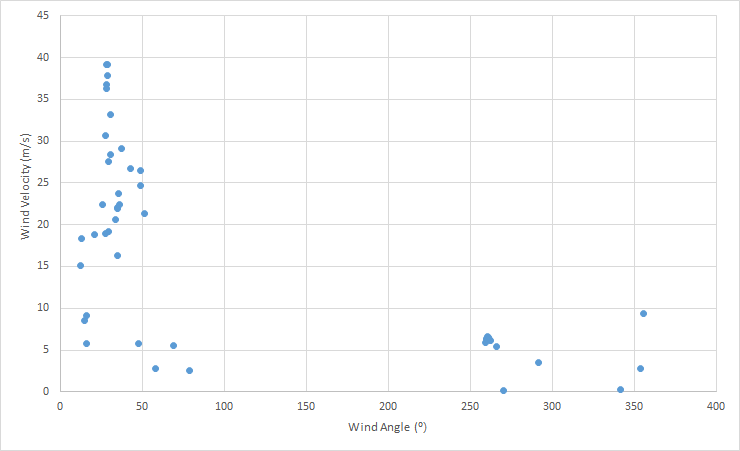
\includegraphics[width=6in]{alan-data.png}
  \caption{Plot of Wind Angle vs. Wind Velocity}
\end{figure}
\section{Data Analysis}
Although the tendencies of the data tend to wary between points, some overarching trends can be noted by analyzing the sign of the first and second derivative (especially where they change).
\section{Excel Formulas}
\end{document}
